\documentclass[]{article}
\usepackage{lmodern}
\usepackage{amssymb,amsmath}
\usepackage{ifxetex,ifluatex}
\usepackage{fixltx2e} % provides \textsubscript
\ifnum 0\ifxetex 1\fi\ifluatex 1\fi=0 % if pdftex
  \usepackage[T1]{fontenc}
  \usepackage[utf8]{inputenc}
\else % if luatex or xelatex
  \ifxetex
    \usepackage{mathspec}
  \else
    \usepackage{fontspec}
  \fi
  \defaultfontfeatures{Ligatures=TeX,Scale=MatchLowercase}
\fi
% use upquote if available, for straight quotes in verbatim environments
\IfFileExists{upquote.sty}{\usepackage{upquote}}{}
% use microtype if available
\IfFileExists{microtype.sty}{%
\usepackage{microtype}
\UseMicrotypeSet[protrusion]{basicmath} % disable protrusion for tt fonts
}{}
\usepackage[margin=1in]{geometry}
\usepackage{hyperref}
\hypersetup{unicode=true,
            pdftitle={What are we learning from language? Associations between gender stereotypes and distributional structure in 25 languages},
            pdfauthor={Molly Lewis and Gary Lupyan},
            pdfborder={0 0 0},
            breaklinks=true}
\urlstyle{same}  % don't use monospace font for urls
\usepackage{graphicx,grffile}
\makeatletter
\def\maxwidth{\ifdim\Gin@nat@width>\linewidth\linewidth\else\Gin@nat@width\fi}
\def\maxheight{\ifdim\Gin@nat@height>\textheight\textheight\else\Gin@nat@height\fi}
\makeatother
% Scale images if necessary, so that they will not overflow the page
% margins by default, and it is still possible to overwrite the defaults
% using explicit options in \includegraphics[width, height, ...]{}
\setkeys{Gin}{width=\maxwidth,height=\maxheight,keepaspectratio}
\IfFileExists{parskip.sty}{%
\usepackage{parskip}
}{% else
\setlength{\parindent}{0pt}
\setlength{\parskip}{6pt plus 2pt minus 1pt}
}
\setlength{\emergencystretch}{3em}  % prevent overfull lines
\providecommand{\tightlist}{%
  \setlength{\itemsep}{0pt}\setlength{\parskip}{0pt}}
\setcounter{secnumdepth}{0}
% Redefines (sub)paragraphs to behave more like sections
\ifx\paragraph\undefined\else
\let\oldparagraph\paragraph
\renewcommand{\paragraph}[1]{\oldparagraph{#1}\mbox{}}
\fi
\ifx\subparagraph\undefined\else
\let\oldsubparagraph\subparagraph
\renewcommand{\subparagraph}[1]{\oldsubparagraph{#1}\mbox{}}
\fi

%%% Use protect on footnotes to avoid problems with footnotes in titles
\let\rmarkdownfootnote\footnote%
\def\footnote{\protect\rmarkdownfootnote}

%%% Change title format to be more compact
\usepackage{titling}

% Create subtitle command for use in maketitle
\providecommand{\subtitle}[1]{
  \posttitle{
    \begin{center}\large#1\end{center}
    }
}

\setlength{\droptitle}{-2em}

  \title{What are we learning from language? Associations between gender
stereotypes and distributional structure in 25 languages}
    \pretitle{\vspace{\droptitle}\centering\huge}
  \posttitle{\par}
  \subtitle{Supplementary Information}
  \author{Molly Lewis and Gary Lupyan}
    \preauthor{\centering\large\emph}
  \postauthor{\par}
      \predate{\centering\large\emph}
  \postdate{\par}
    \date{2020-04-30}

\usepackage{booktabs}
\usepackage{longtable}
\usepackage{array}
\usepackage{multirow}
\usepackage{wrapfig}
\usepackage{float}
\usepackage{colortbl}
\usepackage{pdflscape}
\usepackage{tabu}
\usepackage{threeparttable}
\usepackage{threeparttablex}
\usepackage[normalem]{ulem}
\usepackage{makecell}
\usepackage{xcolor}

\usepackage{float} \usepackage{booktabs}
\floatplacement{figure}{H}

\begin{document}
\maketitle

{
\setcounter{tocdepth}{2}
\tableofcontents
}
\vspace{16pt}

This document was created from an R markdown file. The respository for
the project can be found here:
\url{https://github.com/mllewis/IATLANG/}.

\hypertarget{note-the-si-is-intended-to-be-viewed-interactively-online-at-httpsmollylewis.shinyapps.ioiatlang_si.}{%
\paragraph{\texorpdfstring{NOTE: The SI is intended to be viewed
interactively online at
\url{https://mollylewis.shinyapps.io/iatlang_SI/}.}{NOTE: The SI is intended to be viewed interactively online at https://mollylewis.shinyapps.io/iatlang\_SI/.}}\label{note-the-si-is-intended-to-be-viewed-interactively-online-at-httpsmollylewis.shinyapps.ioiatlang_si.}}

\hypertarget{description-of-iat-data}{%
\section{Description of IAT data}\label{description-of-iat-data}}

As described in the Main Text, the IAT data come from Project Implicit
(\url{https://implicit.harvard.edu/implicit/}; Nosek, Banaji, \&
Greenwald, 2002), for a sample collected 2005 - 2016.

\hypertarget{demographics}{%
\subsection{Demographics}\label{demographics}}

\hypertarget{n-by-country}{%
\subsubsection{N by country}\label{n-by-country}}

Number of participants by country after exclusions. Our final sample
657,335 participants from 39 countries. Participants were exclude who:

\begin{itemize}
\tightlist
\item
  did not have complete gender, country, age, and implicit IAT measures
  (53\%; the majority of these exclusions (69\%) are due to missing IAT
  data - likely cases where the participant started but did not complete
  the IAT task).
\item
  had average latencies for either critical block were over 1,800 ms or
  whose average overall latency was above 1,500 ms (as in Nosek, Banaji,
  \& Greenwald, 2002; 5\% of participants with complete data).
\item
  made excess of 25\% errors in any single critical block (as in Nosek,
  Banaji, \& Greenwald, 2002; 14\% of participants with complete data).
\item
  were from countries with less than 400 participants (1\% of remaining
  participants; in the ``Correlations by language exclusion threshold''
  section below we show analyses with a range of threshold values)
\end{itemize}

\begin{figure}
\centering
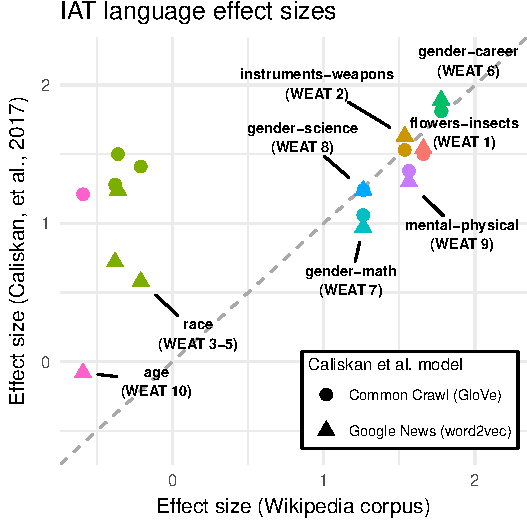
\includegraphics{iatlang_SI_pdf_files/figure-latex/unnamed-chunk-2-1.pdf}
\caption{Note: Data from the US are excluded from this plot because of
the large number of participants (\emph{N} = 638,082).}
\end{figure}

\hypertarget{gender-by-country}{%
\subsubsection{Gender by country}\label{gender-by-country}}

Across countries, there tended to be more female participants, compared
to male participants (\emph{M} = 0.36 proportion males; \emph{SD} =
0.06)

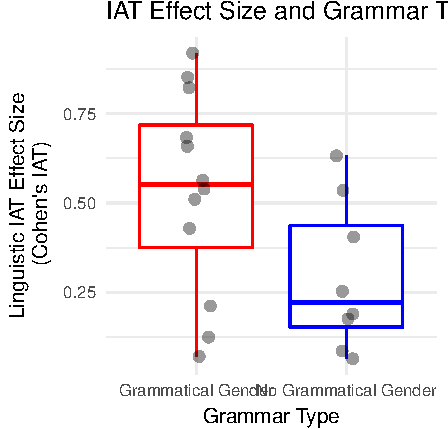
\includegraphics{iatlang_SI_pdf_files/figure-latex/unnamed-chunk-3-1.pdf}

\hypertarget{age-by-country}{%
\subsubsection{Age by country}\label{age-by-country}}

\begin{figure}
\centering
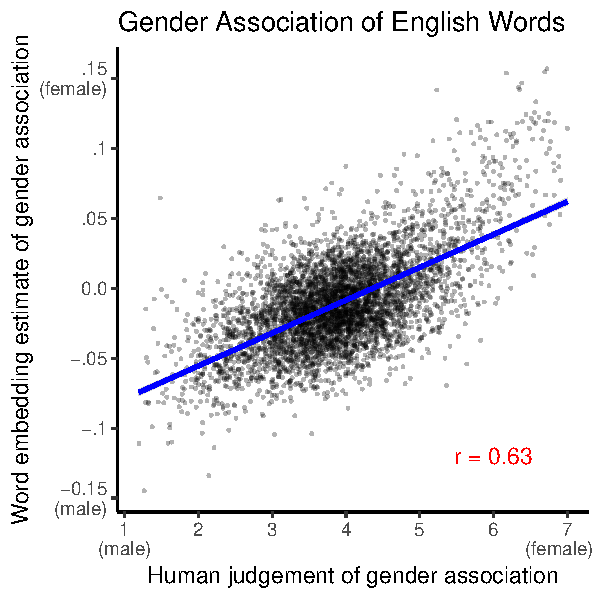
\includegraphics{iatlang_SI_pdf_files/figure-latex/unnamed-chunk-4-1.pdf}
\caption{Bars show mean participant age by country; ranges correspond to
95\% CIs. Red points show median age by country from CIA factbook data.}
\end{figure}

\hypertarget{language-by-country}{%
\subsubsection{Language by country}\label{language-by-country}}

For each country, we identified the language with the most speakers
using Ethnologue (Simons \& Charles, 2018). Note that Ethnologue reports
``Bavarian'' as the primary language of Germany, and ``Daric'' as the
primary language of Afghanistan. In order to map between the other data
sources in our study, we used the more general language variant for
these countries, German and Persian, respectively.

\hypertarget{note-see-online-version-for-this-content-httpsmollylewis.shinyapps.ioiatlang_si}{%
\paragraph{\texorpdfstring{NOTE: See online version for this content
(\url{https://mollylewis.shinyapps.io/iatlang_SI/})}{NOTE: See online version for this content (https://mollylewis.shinyapps.io/iatlang\_SI/)}}\label{note-see-online-version-for-this-content-httpsmollylewis.shinyapps.ioiatlang_si}}

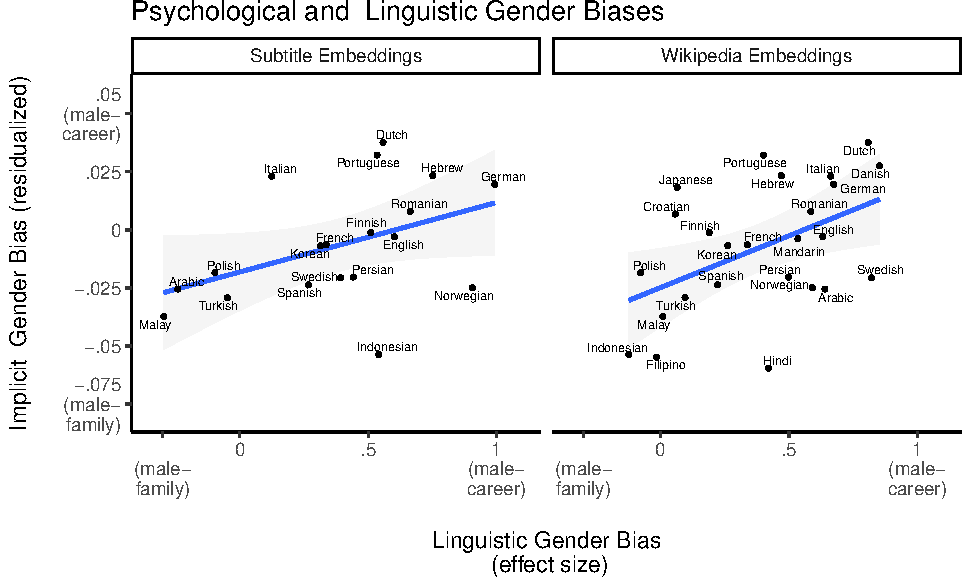
\includegraphics{iatlang_SI_pdf_files/figure-latex/unnamed-chunk-5-1.pdf}
Asterisks correspond to languages that were excluded from our analysis
because word embedding models were unavailable.

\hypertarget{dependent-measures}{%
\subsection{Dependent Measures}\label{dependent-measures}}

Below are histograms for the implicit and explicit measures in the IAT
Project Implicit data presented for each country separately. The
implicit raw scores are the D-score values (estimate of career-gender
association, with positive values indicating strong bias to associate
men with career), and the residualized values are the D-scores with
participant age, participant sex and trial order residualized out. For
the explicit measure, the raw score is the difference between
participants answer to the question, ``How strongly do you associate the
following with males and females?'' for the words ``career'' and for the
word ``family''. Participants indicated their response on a Likert scale
ranging from female (1) to male (7). For each participant, a single
explicit score was calculated as the Career response minus the Family
response, such that greater values indicate a greater bias to associate
males with family. The residualized explicit value is the difference
score with participant age, participant sex and trial order residualized
out (we had no a priori reason for residualizing out trial order for
explicit responses but did so to remain consistent with the residualized
implicit measure).

\hypertarget{note-see-online-version-for-this-content-httpsmollylewis.shinyapps.ioiatlang_si.}{%
\paragraph{\texorpdfstring{NOTE: See online version for this content
(\url{https://mollylewis.shinyapps.io/iatlang_SI/}).}{NOTE: See online version for this content (https://mollylewis.shinyapps.io/iatlang\_SI/).}}\label{note-see-online-version-for-this-content-httpsmollylewis.shinyapps.ioiatlang_si.}}

\hypertarget{implicit}{%
\subsubsection{Implicit}\label{implicit}}

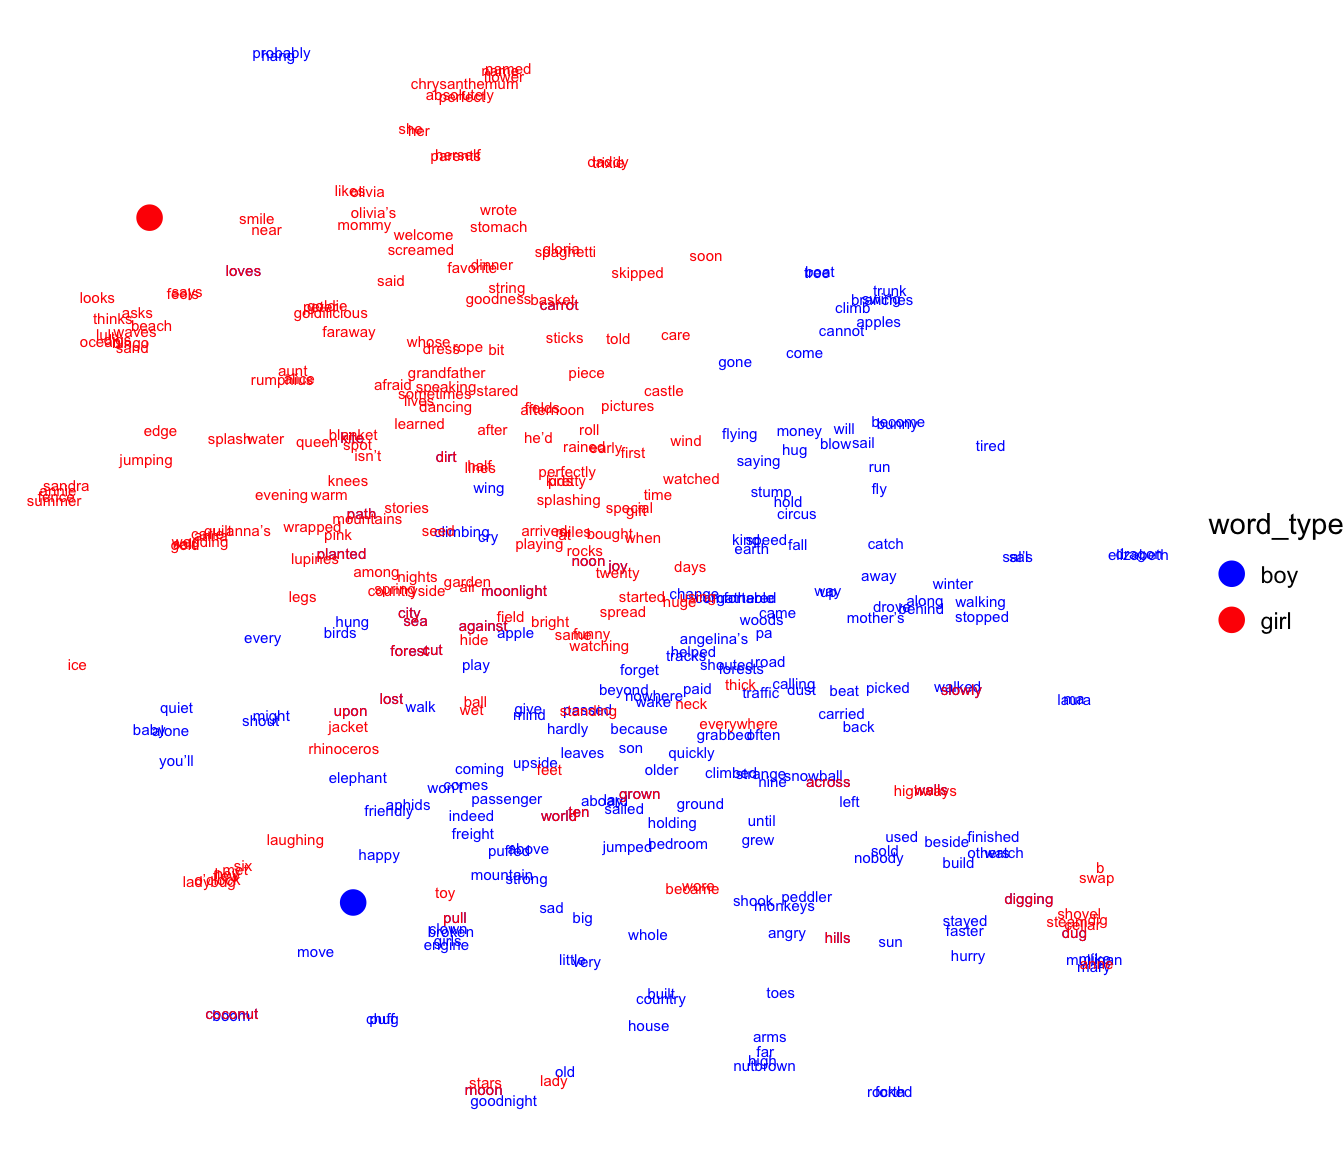
\includegraphics{iatlang_SI_pdf_files/figure-latex/unnamed-chunk-6-1.pdf}

\hypertarget{explicit}{%
\subsubsection{Explicit}\label{explicit}}

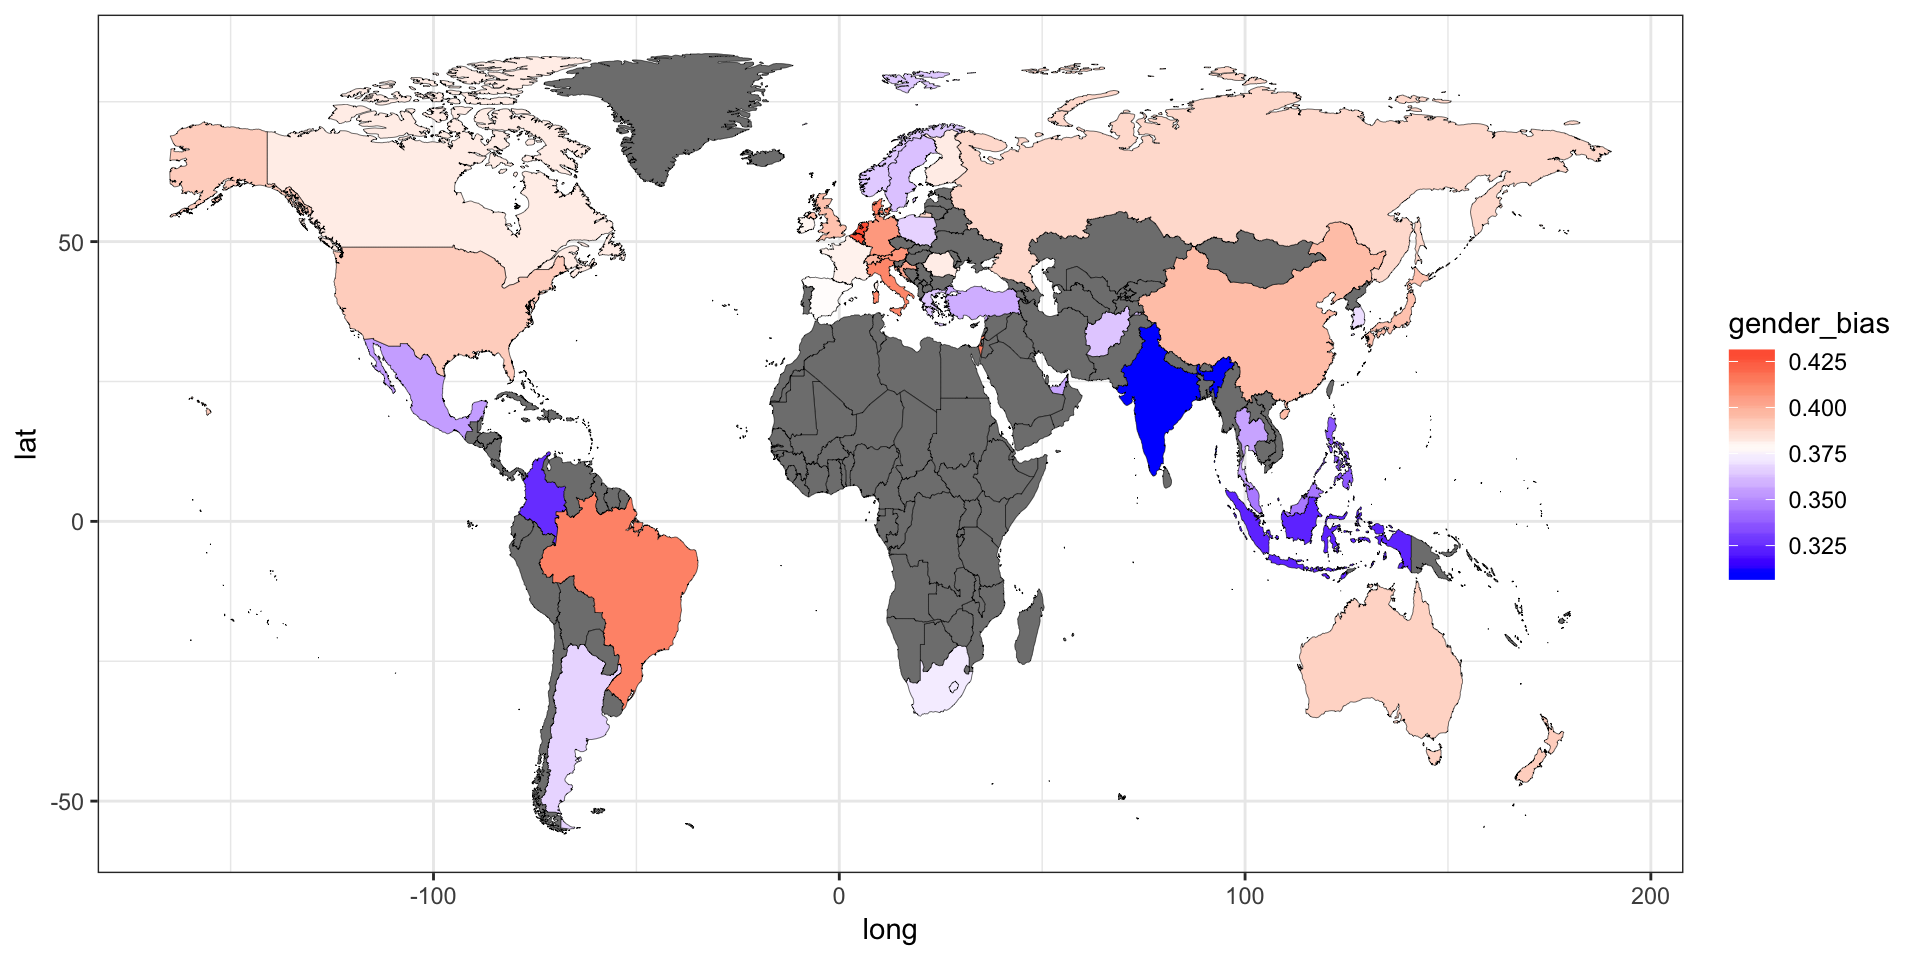
\includegraphics{iatlang_SI_pdf_files/figure-latex/unnamed-chunk-7-1.pdf}

\hypertarget{geographic-distribution-of-iat-scores}{%
\subsection{Geographic distribution of IAT
scores}\label{geographic-distribution-of-iat-scores}}

Residualized implicit career-gender association (IAT score) shown by
country. Larger values (blue) indicate a larger bias to associate men
with the concept of career and women with the concept of family.
Countries in grey correspond to countries for which there was
insufficient data to estimate the country-level career-gender
association. Inset shows IAT scores for European countries only.

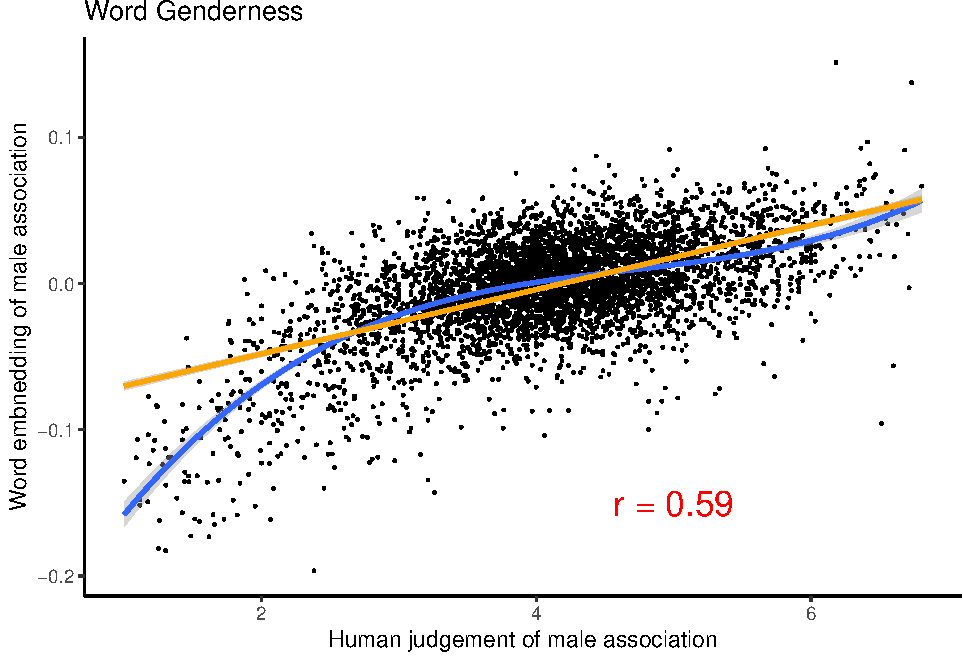
\includegraphics{iatlang_SI_pdf_files/figure-latex/unnamed-chunk-8-1.pdf}

Note that while Hindi is identified as the most frequently spoken
language in India, India is highly multilingual and so Hindi embeddings
may be a poor representation of the linguistic statistics for speakers
in India as a group.

\hypertarget{iat-scores-and-country-age}{%
\subsection{IAT scores and country
age}\label{iat-scores-and-country-age}}

At the participant level, median country age predicts IAT bias over and
above participant age: Countries with older populations tend to have
individuals with stronger career-gender associations, even after
controlling for participant age. The analysis below presents an additive
mixed-effect regression predicting IAT D-score at the participant level
with participant age and median country age, controlling for participant
sex and trial order. The model includes by-country random intercepts.

\begin{table}[H]
\centering
\begin{tabular}{|l|l|l|l|}
\hline

 & \bf{Overall IAT D-score} & &\\ \hline
\bf{Predictors} & Estimates & SE & Statistic \\ \hline
(intercept) & -0.03 & 0.02 & -1.53 \\ \hline
median country age & 0.00 & 0.00 & 4.96 \\ \hline
sex (M) & -0.10 & 0.00 & -103.14 \\ \hline
task order & 0.09 & 0.00 & 105.67 \\ \hline
log age & 0.06 & 0.00 & 55.05 \\ \hline
\bf{Random Effects} \\ \hline
s2 & 0.12 & &\\ \hline
T00 country code & 0.00 & &\\ \hline
ICC & 0.00& & \\ \hline
N country code & 39 & &\\ \hline
\specialrule{.1em}{.05em}{.05em} 
Observations & 657335 & &\\ \hline
Marginal R2 / Conditional R2 & 0.036 / 0.038 & &\\ \hline

\end{tabular}
\end{table}

The relationship between median country age and IAT bias holds, even
after controlling for the percentage women in STEM. The model below
presents an additive mixed effect model predicting IAT D-score at the
participant level with participant age, median country age and
percentage women in STEM in country, controlling for participant sex and
trial order. The model includes by-country random intercepts.

\begin{table}[H]
\centering
\begin{tabular}{|l|l|l|l|}
\hline

 & \bf{Overall IAT D-score} & & \\ \hline
Predictors & Estimates & SE & Statistic \\ \hline
(intercept) & -0.00 & 0.03 & -0.05 \\ \hline
median country age & 0.00 & 0.00 & 4.11 \\ \hline
\% women in STEM & -0.00 & 0.00 & -2.73 \\ \hline
task order & 0.09 & 0.00 & 104.76 \\ \hline
sex (M) & -0.10 & 0.00 & -102.78 \\ \hline
log age & 0.06 & 0.00 & 54.56 \\ \hline
\bf{Random Effects} \\ \hline
s2 & 0.12 & & \\ \hline
T00 country\_code & 0.00 & &\\ \hline
ICC & 0.00 & &\\ \hline
N country\_code & 33& & \\ \hline
\specialrule{.1em}{.05em}{.05em} 

Observations & 646271 & &\\ \hline
Marginal R2 / Conditional R2 & 0.036 / 0.038 & &\\ \hline

\end{tabular}
\end{table}

\hypertarget{study-1b-career-gender-association-across-languages}{%
\section{Study 1b: Career-Gender association across
languages}\label{study-1b-career-gender-association-across-languages}}

\hypertarget{replication-of-caliskan-et-al.-2017}{%
\subsection{Replication of Caliskan et
al.~(2017)}\label{replication-of-caliskan-et-al.-2017}}

Here we replicate the original set of Caliskan, Bryson, and Narayanan
(2017; henceforth \emph{CBN}) findings using the models trained on the
corpora used in our paper, English Wikipedia (Bojanowski, Grave, Joulin,
\& Mikolov, 2016) and Subtitles (Lison \& Tiedemann, 2016; Van Paridon
\& Thompson, 2019).

For both the Wikipedia and Subtitle trained models, we calculate an
effect size for each of the 10 biases reported in CBN which correspond
to behavioral IAT results existing in the literature:
flowers/insects--pleasant/unpleasant,
instruments/weapons--pleasant/unpleasant,
European-American/Afro-American--pleasant/unpleasant,
males/females--career/family, math/arts--male/female,
science/arts--male/female,
mental-disease/physical-disease--permanent/temporary, and
young/old--pleasant/unpleasant (labeled as Word-Embedding Association
Test (WEAT) 1-10 in CBN). Note that CBN test three versions of race
bias. We calculate the bias using the same effect size metric described
in CBN, a standardized difference score of the relative similarity of
the target words to the target attributes (i.e.~relative similarity of
male to career vs.~relative similarity of female to career). This
measure is analogous to the behavioral effect size measure where larger
values indicate larger gender bias.

The figure below shows the effect size measures derived from the English
Wikipedia corpus and the English Subtitle corpus plotted against effect
size estimates reported by CBN from two different models (trained on the
Common Crawl and Google News corpora). With the exception of biases
related to race and age, effect sizes from our corpora are comparable to
those reported by CBN. In particular, for the gender-career IAT---the
bias relevant to our current purposes---we estimate the effect size to
be 1.78, while CBN estimates it as approximately 1.85.

\hypertarget{wikipedia}{%
\subsubsection{Wikipedia}\label{wikipedia}}

\begin{figure}
\centering
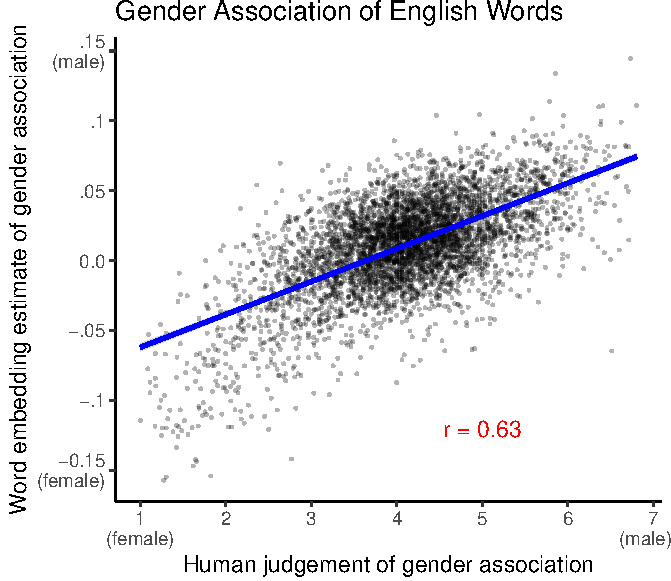
\includegraphics{iatlang_SI_pdf_files/figure-latex/unnamed-chunk-11-1.pdf}
\caption{Effect sizes for the 10 IAT biases types (WEAT 1-10) reported
in Caliskan et al.~(2017; CBN). CBN effect sizes are plotted against
effect sizes derived from the Wikipedia (left) and Subtitle (right)
corpora. Point color corresponds to bias type, and point shape
corresponds to the two CBN models trained on different corpora and with
different algorithms.}
\end{figure}

\hypertarget{subtitles}{%
\subsubsection{Subtitles}\label{subtitles}}

\begin{figure}
\centering
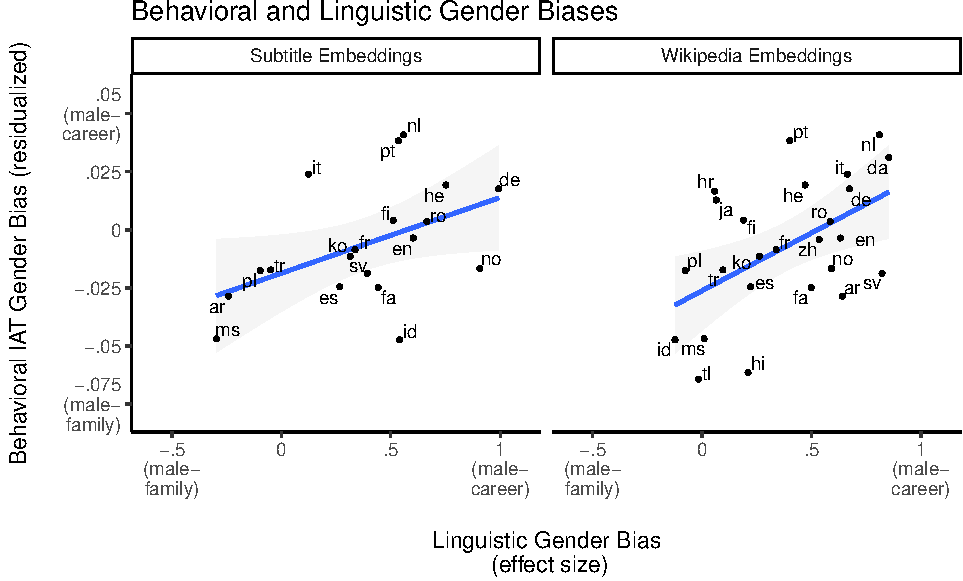
\includegraphics{iatlang_SI_pdf_files/figure-latex/unnamed-chunk-12-1.pdf}
\caption{Effect sizes for the 10 IAT biases types (WEAT 1-10) reported
in Caliskan et al.~(2017; CBN). CBN effect sizes are plotted against
effect sizes derived from the Wikipedia (left) and Subtitle (right)
corpora. Point color corresponds to bias type, and point shape
corresponds to the two CBN models trained on different corpora and with
different algorithms.}
\end{figure}

\hypertarget{descriptive-statistics-for-all-language-level-measures}{%
\subsection{Descriptive statistics for all language-level
measures}\label{descriptive-statistics-for-all-language-level-measures}}

Below are the mean and standard deviation estimates for all measures
presented in Table 1 of the Main Text.

\begin{table}[H]
\centering\begingroup\fontsize{9}{11}\selectfont

\begin{tabular}{l|r|r}
\hline
Measure & Mean & SD\\
\hline
Explicit Male-Career Assoc. & -0.018 & 0.175\\
\hline
Implicit Male-Career Assoc. (IAT) & -0.008 & 0.028\\
\hline
Percent Women in STEM & 14.954 & 4.550\\
\hline
Male-Career Assoc. (Subtitle) & 0.423 & 0.398\\
\hline
Male-Career Assoc. (Wikipedia) & 0.385 & 0.300\\
\hline
Prop. Gendered Occup. Terms & 0.355 & 0.358\\
\hline
Lang. Occup. Genderness (Subtitle) & 0.044 & 0.016\\
\hline
Lang. Occup. Genderness (Wikipedia) & 0.051 & 0.028\\
\hline
Median Country Age & 36.567 & 7.458\\
\hline
\end{tabular}
\endgroup{}
\end{table}

\hypertarget{correlations-by-language-exclusion-threshold}{%
\subsection{Correlations by language exclusion
threshold}\label{correlations-by-language-exclusion-threshold}}

In the Main Text, we report psychological IAT data for participants who
came from countries with at least 400 participants. This cutoff was
largely arbitrary, but was selected to allow for a relatively large
number of languages to be included in our analysis while also excluding
languages with small sample sizes (and therefore less reliable
estimates). Nevertheless, the pattern of findings we report in the Main
Text remains broadly the same when larger thresholds of minimum number
of participants per country are used. The plot below shows pairwise
correlations between the language bias measures and three
psychological/objective measures described in Study 1: Residualized
behavioral IAT, residualized explicit IAT, and percent women in STEM. As
in the main text, the residualized values are participant age,
participant sex, and trial order. Point size corresponds to the number
of languages included in the analysis at that threshold, and point color
corresponds to the \emph{p}-value of the pairwise Pearson's \emph{r}
coefficient.

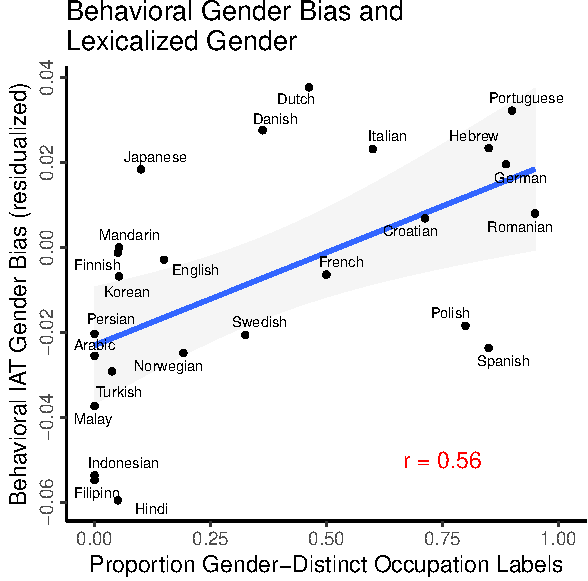
\includegraphics{iatlang_SI_pdf_files/figure-latex/unnamed-chunk-14-1.pdf}

\hypertarget{partial-correlations-controlling-for-median-country-age}{%
\subsection{Partial correlations controlling for median country
age}\label{partial-correlations-controlling-for-median-country-age}}

Partial correlation (Pearson's \emph{r}) for all measures in Study 1 and
2 at the level of languages, controlling for median country age. Single
asterisks indicate \emph{p} \textless{} .05 and double asterisks
indicate \emph{p} \textless{} .01. The + symbol indicates a marginally
significant \emph{p}-value, \emph{p} \textless{} .1.

\begin{table}[H]
\centering\begingroup\fontsize{9}{11}\selectfont

\begin{tabular}{llllllll}
\toprule
\rotatebox{90}{ } & \rotatebox{90}{Explicit Male-Career Assoc.} & \rotatebox{90}{Implicit Male-Career Assoc. (IAT)} & \rotatebox{90}{Percent Women in STEM} & \rotatebox{90}{Male-Career Assoc. (Subtitle)} & \rotatebox{90}{Male-Career Assoc. (Wikipedia)} & \rotatebox{90}{Prop. Gendered Occup. Terms} & \rotatebox{90}{Lang. Occup. Genderness (Subtitle)}\\
\midrule
Explicit Male-Career Assoc. &  & \ .28 & \ .16 & -.06 & \ .38+ & \ .14 & \ .21\\
Implicit Male-Career Assoc. (IAT) & \ .28 &  & -.38+ & \ .42* & \ .43* & \ .48* & \ .31\\
Percent Women in STEM & \ .16 & -.38+ &  & -.49* & -.09 & -.23 & -.10\\
Male-Career Assoc. (Subtitle) & -.06 & \ .42* & -.49* &  & \ .47* & \ .20 & \ .28\\
Male-Career Assoc. (Wikipedia) & \ .38+ & \ .43* & -.09 & \ .47* &  & \ .11 & \ .46*\\
\addlinespace
Prop. Gendered Occup. Terms & \ .14 & \ .48* & -.23 & \ .20 & \ .11 &  & \ .53**\\
Lang. Occup. Genderness (Subtitle) & \ .21 & \ .31 & -.10 & \ .28 & \ .46* & \ .53** & \\
Lang. Occup. Genderness (Wikipedia) & \ .22 & \ .37+ & -.46* & \ .35+ & \ .49* & \ .73** & \ .79**\\
\bottomrule
\end{tabular}
\endgroup{}
\end{table}

\hypertarget{replication-on-untranslated-corpus}{%
\subsection{Replication on untranslated
corpus}\label{replication-on-untranslated-corpus}}

Both the Subtitle and Wikipedia corpora likely contain some documents
that are translated from other languages (e.g., the Wikipedia article on
``Paris'' is written in French and then translated into English). The
parallel content across languages allows us to estimate the gender bias
in language statistics, while holding content constant across languages.
Nevertheless, content may itself be a driver of gender bias (e.g.~one
language may have more articles about male politicians relative to
another).

To understand the contribution of language-specific content on gender
bias, we constructed a corpus of Wikipedia articles in each language
that were originally written in the target language (i.e.,
untranslated). We identified untranslated articles by examining the
\href{https://en.wikipedia.org/wiki/Help:Interlanguage_links}{interlanguage
links} on a Wikipedia article page. These links are pointers to the same
article content in other languages (e.g.~the ``Paris'' article in French
contains a link to the ``Paris'' article in English). Since the original
source language of an article could not be inferred, we excluded all
articles that contained one or more interlanguage links. This ensured
that all remaining articles contained only text originally written in
the target language.

We constructed a corpus for each language containing all untranslated
articles. There were a median of 168,326 articles per language (range:
10,307-14,676,484). We trained fastText (Joulin, et al.~2016) on each
language corpus with default parameters and a dimension size of 200. We
then used these models trained on native text to calculate by-language
IAT bias scores and by-language occupation bias scores, using the same
procedure as with the models described in the Main Text (Studies 1b and
2). One language was excluded following the same exclusion criteria as
in the main analyses (\textgreater= 20\% missing words in model;
Mandarin), but the results remain the same when this language is
included.

Using models trained on the untranslated corpora, we replicate the key
finding from Study 1b showing a positive correlation between the bias
measured behaviorally with the IAT and measured in language (\emph{r} =
.60; \emph{p} = .002; fig below). Notably, the effect size is somewhat
larger relative to the other two corpora types, presumably because
additional bias is introduced by allowing the corpus content to vary
across languages.

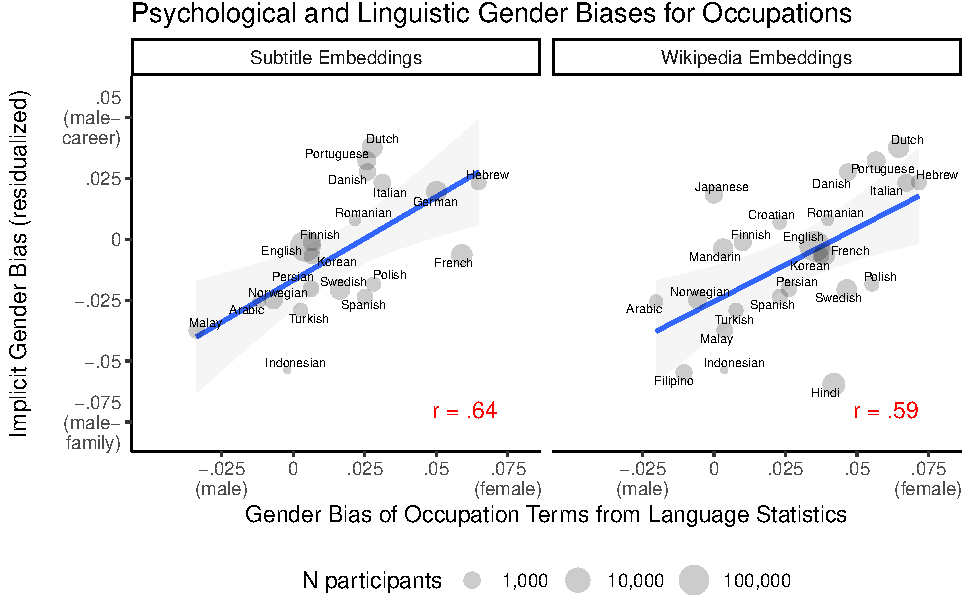
\includegraphics{iatlang_SI_pdf_files/figure-latex/unnamed-chunk-16-1.pdf}

The table below shows the correlation (Pearson's \emph{r}) for all
measures in Study 1 and 2 at the level of languages, including estimates
of language bias obtained from models trained on the untranslated
Wikipedia corpus.

\begin{table}[H]
\centering\begingroup\fontsize{6}{8}\selectfont

\begin{tabular}{llllllllllll}
\toprule
\rotatebox{90}{ } & \rotatebox{90}{Explicit Male-Career Assoc.} & \rotatebox{90}{Implicit Male-Career Assoc. (IAT)} & \rotatebox{90}{Percent Women in STEM} & \rotatebox{90}{Male-Career Assoc. (Subtitle)} & \rotatebox{90}{Male-Career Assoc. (Wikipedia)} & \rotatebox{90}{Male-Career Assoc. (Wikipedia, untranslated)} & \rotatebox{90}{Prop. Gendered Occup. Terms} & \rotatebox{90}{Lang. Occup. Genderness (Subtitle)} & \rotatebox{90}{Lang. Occup. Genderness (Wikipedia)} & \rotatebox{90}{Lang. Occup. Genderness (Wikipedia, untranslated)} & \rotatebox{90}{Median Country Age}\\
\midrule
Explicit Male-Career Assoc. &  & \ .18 & \ .18 & -.08 & \ .34+ & \ .21 & \ .11 & \ .16 & \ .18 & \ .27 & -.07\\
Implicit Male-Career Assoc. (IAT) & \ .18 &  & -.53* & \ .50* & \ .48* & \ .60** & \ .57** & \ .49* & \ .49* & \ .60** & \ .61**\\
Percent Women in STEM & \ .18 & -.53* &  & -.55* & -.19 & -.39+ & -.35 & -.26 & -.53* & -.44* & -.42+\\
Male-Career Assoc. (Subtitle) & -.08 & \ .50* & -.55* &  & \ .51* & \ .49* & \ .28 & \ .38 & \ .41+ & \ .45* & \ .31\\
Male-Career Assoc. (Wikipedia) & \ .34+ & \ .48* & -.19 & \ .51* &  & \ .90** & \ .18 & \ .51* & \ .53** & \ .47* & \ .25\\
\addlinespace
Male-Career Assoc.
(Wikipedia, untranslated) & \ .21 & \ .60** & -.39+ & \ .49* & \ .90** &  & \ .23 & \ .35 & \ .52** & \ .46* & \ .48*\\
Prop. Gendered Occup. Terms & \ .11 & \ .57** & -.35 & \ .28 & \ .18 & \ .23 &  & \ .60** & \ .77** & \ .75** & \ .35+\\
Lang. Occup. Genderness (Subtitle) & \ .16 & \ .49* & -.26 & \ .38 & \ .51* & \ .35 & \ .60** &  & \ .81** & \ .74** & \ .44+\\
Lang. Occup. Genderness (Wikipedia) & \ .18 & \ .49* & -.53* & \ .41+ & \ .53** & \ .52** & \ .77** & \ .81** &  & \ .83** & \ .34+\\
Lang. Occup. Genderness
(Wikipedia, untranslated) & \ .27 & \ .60** & -.44* & \ .45* & \ .47* & \ .46* & \ .75** & \ .74** & \ .83** &  & \ .48*\\
\addlinespace
Median Country Age & -.07 & \ .61** & -.42+ & \ .31 & \ .25 & \ .48* & \ .35+ & \ .44+ & \ .34+ & \ .48* & \\
\bottomrule
\end{tabular}
\endgroup{}
\end{table}

Single asterisks indicate \(p\) \textless{} .05 and double asterisks
indicate \(p\) \textless{} .01. The + symbol indicates a marginally
significant \(p\)-value, \(p\) \textless{} .1

\hypertarget{study-1c-pre-registered-analysis-of-british-vs.-american-english}{%
\section{Study 1c: Pre-registered Analysis of British vs.~American
English}\label{study-1c-pre-registered-analysis-of-british-vs.-american-english}}

The pre-registration to this study can be found here:
\url{https://osf.io/3f9ed}.

\hypertarget{iat-target-words}{%
\subsection{IAT Target Words}\label{iat-target-words}}

Presented below are the target words for each of the 31 IATs used in our
analyses. Each IAT has two target categories (e.g.~``money'' and
``love'') and two attribute categories (e.g.~negative and positive).

\begin{table}[H]
\centering\begingroup\fontsize{7}{9}\selectfont

\begin{tabular}{l|l}
\hline
IAT & items\\
\hline
Athletic People - Intelligent People & \makecell[l]{CATEGORY 1:  fit, active, nimble, energetic, muscular \\ CATEGORY 2:  clever, bright, smart, brilliant, intellectual, academic \\ ATTRIBUTE 1:  animosity, dirty, evil, gross, neglected, rotten \\ ATTRIBUTE 2:  appealing, delight, excitement, glee, laughing, splendid \\}\\
\hline
Avoiding - Approaching & \makecell[l]{CATEGORY 1:  back, withdraw, retreat, away \\ CATEGORY 2:  toward, closer, advance, forward, near \\ ATTRIBUTE 1:  failure, horrendous, nasty, repulsive \\ ATTRIBUTE 2:  adore, cheerful, friendship, joyful, smiling \\}\\
\hline
Career - Family & \makecell[l]{CATEGORY 1:  work, business, job, profession, office \\ CATEGORY 2:  home, household, children, domestic, kitchen \\ ATTRIBUTE 1:  failure, horrendous, nasty, repulsive \\ ATTRIBUTE 2:  adore, cheerful, friendship, joyful, smiling \\}\\
\hline
Chaos - Order & \makecell[l]{CATEGORY 1:  anarchy, scattered, disarray, random \\ CATEGORY 2:  control, predictable, discipline, structure \\ ATTRIBUTE 1:  annoy, disaster, grotesque, horrific \\ ATTRIBUTE 2:  attractive, delightful, fabulous, glorious, pleasing \\}\\
\hline
Cold - Hot & \makecell[l]{CATEGORY 1:  cool, freeze, frozen, ice, chill \\ CATEGORY 2:  warm, boil, heat, steam, burn \\ ATTRIBUTE 1:  abuse, bomb, grief, pain, poison, sadness \\ ATTRIBUTE 2:  cheer, friend, love, paradise, pleasure, splendid \\}\\
\hline
Determinism - Free Will & \makecell[l]{CATEGORY 1:  arranged, destined, fixed \\ CATEGORY 2:  choice, intention, freedom \\ ATTRIBUTE 1:  annoy, disaster, grotesque, horrific \\ ATTRIBUTE 2:  attractive, delightful, fabulous, glorious, pleasing \\}\\
\hline
Friends - Family & \makecell[l]{CATEGORY 1:  chum, buddy, pal, peers, companion \\ CATEGORY 2:  mother, father, siblings, child \\ ATTRIBUTE 1:  awful, disgust, hate, selfish, tragic \\ ATTRIBUTE 2:  beautiful, fantastic, happy, lovely, pleasure, terrific \\}\\
\hline
Helpers - Leaders & \makecell[l]{CATEGORY 1:  assistant, worker, attendant, employee \\ CATEGORY 2:  president, boss, manage, senator \\ ATTRIBUTE 1:  hatred, hurtful, sickening \\ ATTRIBUTE 2:  celebrate, enjoy, favorable, gorgeous, magnificent, triumph \\}\\
\hline
Innocence - Wisdom & \makecell[l]{CATEGORY 1:  simple, pure, naive, inexperience, youthful \\ CATEGORY 2:  mature, knowledge, enlightened, sophisticated \\ ATTRIBUTE 1:  awful, disgust, hate, selfish, tragic \\ ATTRIBUTE 2:  beautiful, fantastic, happy, lovely, pleasure, terrific \\}\\
\hline
Jocks - Nerds & \makecell[l]{CATEGORY 1:  sports, strong, athletic, exercise, football, muscles \\ CATEGORY 2:  intelligent, smart, study, calculator, brains \\ ATTRIBUTE 1:  failure, horrendous, nasty, repulsive \\ ATTRIBUTE 2:  adore, cheerful, friendship, joyful, smiling \\}\\
\hline
Lawyers - Politicians & \makecell[l]{CATEGORY 1:  attorney, counsel, prosecution \\ CATEGORY 2:  mayor, senator, governor, representative \\ ATTRIBUTE 1:  hatred, hurtful, sickening \\ ATTRIBUTE 2:  celebrate, enjoy, favorable, gorgeous, magnificent, triumph \\}\\
\hline
Money - Love & \makecell[l]{CATEGORY 1:  wealth, investments, cash \\ CATEGORY 2:  affection, heart, relationship, romance \\ ATTRIBUTE 1:  failure, horrendous, nasty, repulsive \\ ATTRIBUTE 2:  adore, cheerful, friendship, joyful, smiling \\}\\
\hline
National Defense - Education & \makecell[l]{CATEGORY 1:  military, soldiers, combat, army, navy, marines \\ CATEGORY 2:  educate, schools, teachers, books, teach, students \\ ATTRIBUTE 1:  annoy, disaster, grotesque, horrific \\ ATTRIBUTE 2:  attractive, delightful, fabulous, glorious, pleasing \\}\\
\hline
Organized Labor - Management & \makecell[l]{CATEGORY 1:  union, workers, employees, staff \\ CATEGORY 2:  supervisors, boss, administration, employer, managers \\ ATTRIBUTE 1:  hatred, hurtful, sickening \\ ATTRIBUTE 2:  celebrate, enjoy, favorable, gorgeous, magnificent, triumph \\}\\
\hline
Poor People - Rich People & \makecell[l]{CATEGORY 1:  poor, impoverished, broke, bankrupt \\ CATEGORY 2:  wealthy, affluent, prosperous \\ ATTRIBUTE 1:  animosity, dirty, evil, gross, neglected, rotten \\ ATTRIBUTE 2:  appealing, delight, excitement, glee, laughing, splendid \\}\\
\hline
Private - Public & \makecell[l]{CATEGORY 1:  personal, confidential, secret, secluded \\ CATEGORY 2:  communal, accessible, open \\ ATTRIBUTE 1:  awful, disgust, hate, selfish, tragic \\ ATTRIBUTE 2:  beautiful, fantastic, happy, lovely, pleasure, terrific \\}\\
\hline
\end{tabular}
\endgroup{}
\end{table}

\begin{table}[H]
\centering\begingroup\fontsize{7}{9}\selectfont

\begin{tabular}{l|l}
\hline
IAT & items\\
\hline
Protein - Carbohydrates & \makecell[l]{CATEGORY 1:  beef, chicken, eggs, fish, meat \\ CATEGORY 2:  pasta, bread, starch, cereal, grains, rice \\ ATTRIBUTE 1:  awful, disgust, hate, selfish, tragic \\ ATTRIBUTE 2:  beautiful, fantastic, happy, lovely, pleasure, terrific \\}\\
\hline
Punishment - Forgiveness & \makecell[l]{CATEGORY 1:  penalty, retribution, discipline, punitive, sanction \\ CATEGORY 2:  pardon, reprieve, amnesty, mercy \\ ATTRIBUTE 1:  hatred, hurtful, sickening \\ ATTRIBUTE 2:  celebrate, enjoy, favorable, gorgeous, magnificent, triumph \\}\\
\hline
Rebellious - Conforming & \makecell[l]{CATEGORY 1:  question, challenge, defy, resist \\ CATEGORY 2:  follow, obey, yield, comply, abide \\ ATTRIBUTE 1:  angry, ghastly, horrible, negative, ugly \\ ATTRIBUTE 2:  cherish, excellent, glad, spectacular \\}\\
\hline
Rich People - Beautiful People & \makecell[l]{CATEGORY 1:  wealthy, prosperous, affluent \\ CATEGORY 2:  handsome, gorgeous, stunning, attractive \\ ATTRIBUTE 1:  angry, ghastly, horrible, negative, ugly \\ ATTRIBUTE 2:  cherish, excellent, glad, spectacular \\}\\
\hline
Security - Freedom & \makecell[l]{CATEGORY 1:  safe, secure, controlled, protected \\ CATEGORY 2:  free, liberty, independent \\ ATTRIBUTE 1:  angry, ghastly, horrible, negative, ugly \\ ATTRIBUTE 2:  cherish, excellent, glad, spectacular \\}\\
\hline
Skeptical - Trusting & \makecell[l]{CATEGORY 1:  questioning, hesitant, wary, doubtful \\ CATEGORY 2:  convinced, confident, accepting, believing \\ ATTRIBUTE 1:  animosity, dirty, evil, gross, neglected, rotten \\ ATTRIBUTE 2:  appealing, delight, excitement, glee, laughing, splendid \\}\\
\hline
Speed - Accuracy & \makecell[l]{CATEGORY 1:  fast, swift, rapid, quick, speedy \\ CATEGORY 2:  correct, accurate, precise, valid, exact \\ ATTRIBUTE 1:  abuse, bomb, grief, pain, poison, sadness \\ ATTRIBUTE 2:  cheer, friend, love, paradise, pleasure, splendid \\}\\
\hline
Stable - Flexible & \makecell[l]{CATEGORY 1:  same, familiar, steady, fixed, enduring, permanent \\ CATEGORY 2:  shifting, new, different, variable, changing, novelty, fluctuate \\ ATTRIBUTE 1:  awful, disgust, hate, selfish, tragic \\ ATTRIBUTE 2:  beautiful, fantastic, happy, lovely, pleasure, terrific \\}\\
\hline
State - Church & \makecell[l]{CATEGORY 1:  government, republic, nation, constitution \\ CATEGORY 2:  religion, spirituality, faith, scripture \\ ATTRIBUTE 1:  animosity, dirty, evil, gross, neglected, rotten \\ ATTRIBUTE 2:  appealing, delight, excitement, glee, laughing, splendid \\}\\
\hline
Tall People - Short People & \makecell[l]{CATEGORY 1:  big, large, gigantic, towering \\ CATEGORY 2:  small, tiny, little, slight, petite \\ ATTRIBUTE 1:  awful, disgust, hate, selfish, tragic \\ ATTRIBUTE 2:  beautiful, fantastic, happy, lovely, pleasure, terrific \\}\\
\hline
Team - Individual & \makecell[l]{CATEGORY 1:  squad, players, group, bunch \\ CATEGORY 2:  person, autonomous, solo, one \\ ATTRIBUTE 1:  awful, disgust, hate, selfish, tragic \\ ATTRIBUTE 2:  beautiful, fantastic, happy, lovely, pleasure, terrific \\}\\
\hline
Technology - Nature & \makecell[l]{CATEGORY 1:  machines, innovation, devices, invention \\ CATEGORY 2:  animals, natural, plants, living \\ ATTRIBUTE 1:  annoy, disaster, grotesque, horrific \\ ATTRIBUTE 2:  attractive, delightful, fabulous, glorious, pleasing \\}\\
\hline
Tradition - Progress & \makecell[l]{CATEGORY 1:  ritual, custom, convention, stability \\ CATEGORY 2:  development, advancement, innovation, change \\ ATTRIBUTE 1:  angry, ghastly, horrible, negative, ugly \\ ATTRIBUTE 2:  cherish, excellent, glad, spectacular \\}\\
\hline
Urban - Rural & \makecell[l]{CATEGORY 1:  city, busy, noise, buildings \\ CATEGORY 2:  country, farm, slow, quiet, fields \\ ATTRIBUTE 1:  annoy, disaster, grotesque, horrific \\ ATTRIBUTE 2:  attractive, delightful, fabulous, glorious, pleasing \\}\\
\hline
Winter - Summer & \makecell[l]{CATEGORY 1:  january, cold, february, december \\ CATEGORY 2:  june, hot, july, august \\ ATTRIBUTE 1:  annoy, disaster, grotesque, horrific \\ ATTRIBUTE 2:  attractive, delightful, fabulous, glorious, pleasing \\}\\
\hline
\end{tabular}
\endgroup{}
\end{table}

\hypertarget{behavioral-data-exclusion-criteria}{%
\subsection{Behavioral data exclusion
criteria}\label{behavioral-data-exclusion-criteria}}

We excluded participants using the pre-defined criteria in the AIID
dataset, described below. Participants were excluded if any one of the
seven criteria were not satisfied.

\begin{enumerate}
\def\labelenumi{\arabic{enumi}.}
\tightlist
\item
  \(>\)= 35\% responses \(<\) 300ms responses in any one practice block.
\item
  \(>\)= 25\% responses \(<\) 300ms responses in any one critical block.
\item
  \(>\)= 10\% responses \(<\) 300ms in critical blocks.
\item
  \(>\)= 50\% error rate in any one practice block.
\item
  \(>\)= 40\% error rate in practice blocks.
\item
  \(>\)= 40\% error rate in any one critical block.
\item
  \(>\)= 30\% error rate in critical blocks.
\end{enumerate}

\hypertarget{pre-registered-model}{%
\subsection{Pre-registered model}\label{pre-registered-model}}

The exact pre-registered analysis (\url{https://osf.io/3f9ed/}) of Study
1c is presented below. Pairwise correlations between all variables
(language bias, behavioral bias, and UK-US difference measures) are
shown, averaging across estimates of language bias from the 5 model
runs. Error bars are 95\% CIs. As stated in the pre-registration, the
key test of our hypothesis is that the correlation between the UK - US
linguistic difference (``Language Bias Difference'') and the UK - US
behavioral difference (``Behavioral Bias Difference'') is greater than 0
(shown in red below). That data are consistent with this prediction.

The confirmatory dataset is shown on the right, along with the smaller
exploratory dataset on the left for reference.

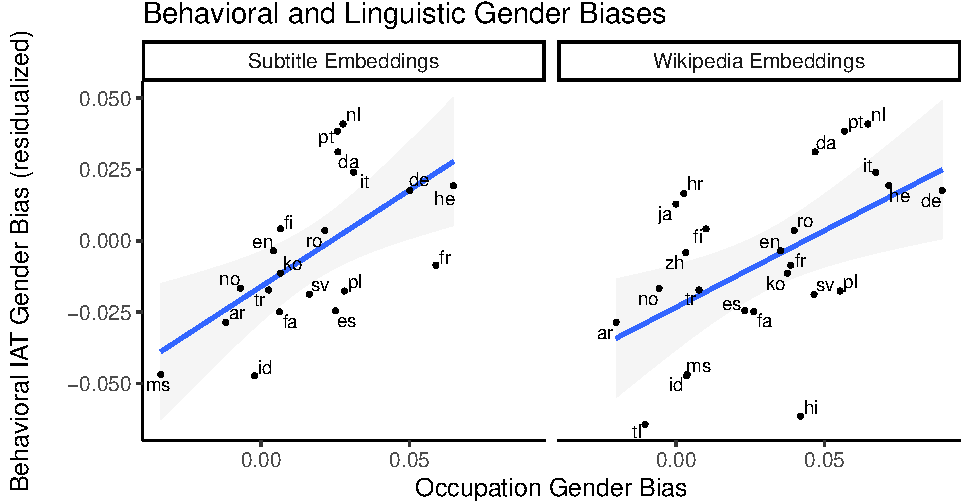
\includegraphics{iatlang_SI_pdf_files/figure-latex/unnamed-chunk-19-1.pdf}

\hypertarget{mixed-effect-model}{%
\subsection{Mixed-effect model}\label{mixed-effect-model}}

The full results to the mixed-effect model described in the paper are
presented below:

\begin{table}[H]
\centering
\begin{tabular}{|l|l|l|l|}
\hline

& \bf{Behavioral Effect Resid} & & \\ \hline
\bf{Predictors} & Estimates & SE & Statistic \\ \hline
(intercept) & -0.00 & 0.05 & -0.09 \\ \hline
country (uk) & 0.02 & 0.01 & 1.74 \\ \hline
language bias difference (uk - us) & -0.03 & 0.07 & -0.42 \\ \hline
country:language bias difference & 0.05 & 0.02 & 2.88 \\ \hline
\bf{Random Effects} \\ \hline
s2 & 0.20  & & \\ \hline
T00 user id & 0.01  & & \\ \hline
T00 domain & 0.07 & &  \\ \hline
ICC & 0.27  & & \\ \hline
N user id & 22059  & & \\ \hline
N domain & 31  & & \\ \hline
\specialrule{.1em}{.05em}{.05em} 
Observations & 27045  & & \\ \hline
Marginal R2 / Conditional R2 & 0.001 / 0.273 \\ \hline

\end{tabular}
\end{table}

\hypertarget{study-2-gender-association-and-lexicalized-gender}{%
\section{Study 2: Gender association and lexicalized
gender}\label{study-2-gender-association-and-lexicalized-gender}}

\hypertarget{note-see-online-version-for-this-content-httpsmollylewis.shinyapps.ioiatlang_si.-1}{%
\paragraph{\texorpdfstring{NOTE: See online version for this content
(\url{https://mollylewis.shinyapps.io/iatlang_SI/}).}{NOTE: See online version for this content (https://mollylewis.shinyapps.io/iatlang\_SI/).}}\label{note-see-online-version-for-this-content-httpsmollylewis.shinyapps.ioiatlang_si.-1}}

\hypertarget{grammatical-gender-coding}{%
\subsection{Grammatical gender coding}\label{grammatical-gender-coding}}

Below is the binary coding (gender vs.~no gender) of each language for a
sex-based grammatical gender system, based on WALS (Dryer \& Haspelmath,
2013) and other sources when information was not available from WALS.

\includegraphics{iatlang_SI_pdf_files/figure-latex/unnamed-chunk-21-1.pdf}

\hypertarget{occupation-items}{%
\subsection{Occupation Items}\label{occupation-items}}

In Study 2, we selected 20 occupation labels from the set of items used
in Misersky, et al.~(2014). Listed below are the 20 items along with
their perceived gender bias as reported in Misersky, et al.~(2014;
larger values indicate occupation is perceived to be more closely
associated with women).

\includegraphics{iatlang_SI_pdf_files/figure-latex/unnamed-chunk-22-1.pdf}

\hypertarget{occupation-translations}{%
\subsection{Occupation Translations}\label{occupation-translations}}

Below are the translations of the 20 occupation words for each of the 25
target languages. ``Translation ID'' identifies the translation when
multiple translations were provided for a given occupation/language.

\includegraphics{iatlang_SI_pdf_files/figure-latex/unnamed-chunk-23-1.pdf}

\hypertarget{predicting-career-gender-association-with-both-language-measures}{%
\subsection{Predicting career-gender association with both language
measures}\label{predicting-career-gender-association-with-both-language-measures}}

In this analysis, we predict the magnitude of implicit career-gender
association by language with an additive linear model. As predictors, we
include proportion gender distinct labels and linguistic career-gender
association (as measured by word embeddings of the IAT words). Model
coefficients are shown below for models based on the Subtitle (top) and
Wikipedia (bottom) corpora.

Subtitle Corpus:

\begin{table}[H]
\centering\begingroup\fontsize{9}{11}\selectfont

\begin{tabular}{l|r|r|r|r}
\hline
term & estimate & std.error & statistic & p.value\\
\hline
(Intercept) & 0.108 & 0.157 & 0.691 & 0.498\\
\hline
Prop. Gendered Occupuation Terms & 0.388 & 0.164 & 2.364 & 0.029\\
\hline
Lang. Male-Career Assoc (Subtitle) & 0.332 & 0.165 & 2.011 & 0.059\\
\hline
\end{tabular}
\endgroup{}
\end{table}

This model accounts for 40.63\% variance.

Wikipedia Corpus:

\begin{table}[H]
\centering\begingroup\fontsize{9}{11}\selectfont

\begin{tabular}{l|r|r|r|r}
\hline
term & estimate & std.error & statistic & p.value\\
\hline
(Intercept) & 0.000 & 0.154 & 0.000 & 1.000\\
\hline
Prop. Gendered Occupuation Terms & 0.520 & 0.159 & 3.270 & 0.004\\
\hline
Lang. Male-Career Assoc (Wikipedia) & 0.363 & 0.159 & 2.282 & 0.033\\
\hline
\end{tabular}
\endgroup{}
\end{table}

This model accounts for 45.32\% variance.

Presented below are models that include median country age as an
additional predictor.

Subtitle Corpus:

\begin{table}[H]
\centering\begingroup\fontsize{9}{11}\selectfont

\begin{tabular}{l|r|r|r|r}
\hline
term & estimate & std.error & statistic & p.value\\
\hline
(Intercept) & 0.078 & 0.150 & 0.521 & 0.609\\
\hline
Prop. Gendered Occupuation Terms & 0.328 & 0.159 & 2.063 & 0.054\\
\hline
Lang. Male-Career Assoc (Subtitle) & 0.270 & 0.160 & 1.681 & 0.110\\
\hline
Median Country Age & 0.298 & 0.168 & 1.776 & 0.093\\
\hline
\end{tabular}
\endgroup{}
\end{table}

This model accounts for 49.48\% variance.

Wikipedia Corpus:

\begin{table}[H]
\centering\begingroup\fontsize{9}{11}\selectfont

\begin{tabular}{l|r|r|r|r}
\hline
term & estimate & std.error & statistic & p.value\\
\hline
(Intercept) & 0.000 & 0.135 & 0.000 & 1.000\\
\hline
Prop. Gendered Occupuation Terms & 0.385 & 0.148 & 2.606 & 0.017\\
\hline
Lang. Male-Career Assoc (Wikipedia) & 0.297 & 0.142 & 2.095 & 0.049\\
\hline
Median Country Age & 0.413 & 0.150 & 2.758 & 0.012\\
\hline
\end{tabular}
\endgroup{}
\end{table}

This model accounts for 59.85\% variance.

\hypertarget{gender-associations-in-language-and-other-psychological-measures}{%
\section{Gender associations in language and other psychological
measures}\label{gender-associations-in-language-and-other-psychological-measures}}

Several recent studies (Falk \& Hermle, 2018; Stoet \& Geary, 2018) have
presented novel theories to account for cases of structural inequality
related to gender. Both of these papers argue that psychological
differences play a causal role in the emergence of structural
inequality. Here, we show that degree of gender bias in language is
correlated with these psychological differences at the country level,
consistent with the idea that language experience could be playing a
causal role in the emergence of psychological differences.

\hypertarget{falk-and-hermle-2018}{%
\subsection{Falk and Hermle (2018)}\label{falk-and-hermle-2018}}

Gender differences in preferences (Falk \& Hermle, 2018; composite score
of ``six fundamental preferences with regard to social and nonsocial
domains: willingness to take risks; patience, which captures preferences
over the intertemporal timing of rewards; altruism; trust; and positive
and negative reciprocity, which capture the costly willingness to reward
kind actions or to punish unkind actions, respectively.'') as a function
of linguistic gender bias measured in the Subtitle corpus. These two
measures are correlated (\emph{r}(25) = 0.48 {[}0.12, 0.73{]}, \emph{p}
= 0.01): Countries with greater differences in gender preferences also
have greater gender bias present in their languages.

\includegraphics{iatlang_SI_pdf_files/figure-latex/unnamed-chunk-29-1.pdf}

We also find that per capita GDP (World Bank database; 2017 GDP per
capita (current US\$ indicator) is correlated with linguistic gender
bias measured in both corpora (Wikipedia: \emph{r}(35) = 0.64 {[}0.4,
0.8{]}, \emph{p} \textless{} .0001; Subtitle: \emph{r}(31) = 0.58
{[}0.29, 0.77{]}, \emph{p} \textless{} .001). Futher, the magnitude of
the male-career association in the language spoken in a country predicts
the magnitude of that bias measured via the behavioral IAT, controlling
for both national GDP and median country age. Results are presented
below for mixed-effect models predicting behavioral IAT at the country
level with median country age, GDP, and Language IAT as fixed effects,
and random intercepts by language.

Wikipedia Corpus:

\begin{tabular}{l|r|r|r}
\hline
term & estimate & std.error & statistic\\
\hline
(Intercept) & -0.02 & 0.01 & -2.11\\
\hline
Lang. Male-Career Assoc (Wikipedia) & 0.04 & 0.01 & 2.42\\
\hline
GDP & 0.00 & 0.00 & -1.07\\
\hline
Median Country Age & 0.02 & 0.00 & 3.66\\
\hline
\end{tabular}

Subtitle Corpus:

\begin{tabular}{l|r|r|r}
\hline
term & estimate & std.error & statistic\\
\hline
(Intercept) & -0.01 & 0.01 & -1.72\\
\hline
Lang. Male-Career Assoc (Subtitle) & 0.03 & 0.01 & 1.97\\
\hline
GDP & 0.00 & 0.00 & -0.32\\
\hline
Median Country Age & 0.01 & 0.01 & 2.10\\
\hline
\end{tabular}

\hypertarget{stoet-and-geary-2018}{%
\subsection{Stoet and Geary (2018)}\label{stoet-and-geary-2018}}

Gender difference in STEM Self Efficacy (Stoet \& Geary, 20178; ``The
sex difference in self efficacy (boys -- girls)'') as a function of
linguistic gender bias measured in the Subtitle corpus. These two
measures are correlated (\emph{r}(28) = 0.59 {[}0.3, 0.79{]}, \emph{p}
\textless{} .001): Countries with greater gender differences in
self-efficacy also have greater gender bias present in their languages.
Futher, self-efficacy mediated the effect of language statistics on
percentage of women in stem (path-ab = -0.33; \emph{p} = 0.01),
suggesting that language statistics could be critical causal factor
underlying gender differences in STEM participation.

\includegraphics{iatlang_SI_pdf_files/figure-latex/unnamed-chunk-34-1.pdf}

\hypertarget{references}{%
\section{References}\label{references}}

Benesty, M. (2018). fastrtext: `fastText' Wrapper for Text
Classification and Word Representation (R package version 0.2.5).
\url{https://CRAN.R-project.org/package=fastrtext/}

Bojanowski, P., Grave, E., Joulin, A., \& Mikolov, T. (2016). Enriching
word vectors with subword information.
\url{https://arxiv.org/abs/1607.04606}

Caliskan, A., Bryson, J. J., \& Narayanan, A. (2017). Semantics derived
automatically from language corpora contain human-like biases.
\emph{Science}, \emph{356}(6334), 183--186.

Dryer, M. S., \& Haspelmath, M. (Eds.). (2013). \emph{WALS online}.
Leipzig: Max Planck Institute for Evolutionary Anthropology. Retrieved
from \url{http://wals.info/}

Falk, A., \& Hermle, J. (2018). Relationship of gender differences in
preferences to economic development and gender equality. \emph{Science},
362 (6412), eaas9899.

Joulin A, Grave E, Bojanowski P, \& Mikolov T (2016) Bag of tricks for
efficient text classification. \emph{818arXiv preprint
arXiv:1607.01759)}

Lison, P., \& Tiedemann, J. (2016). OpenSubtitles2016: Extracting large
parallel corpora from movie and TV subtitles. In \emph{Proceedings of
the 10th International Conference on Language Resources and Evaluation}.

Misersky, J., Gygax, P. M., Canal, P., Gabriel, U., Garnham, A., Braun,
F., . . . others. (2014). Norms on the gender perception of role nouns
in Czech, English, French, German, Italian, Norwegian, and Slovak.
\emph{Behavior Research Methods}, \emph{46}(3), 841--871.

Nosek, B. A., Banaji, M. R., \& Greenwald, A. G. (2002). Harvesting
implicit group attitudes and beliefs from a demonstration web site.
\emph{Group Dynamics: Theory, Research, and Practice}, \emph{6}(1), 101.

Simons, G. F., \& Charles, D. F. (Eds.). (2018). Ethnologue: Languages
of the world. Dallas, Texas: Online version:
\url{http://www.ethnologue.com}. SIL International.

Stoet, G., \& Geary, D. C. (2018). The gender-equality paradox in
science, technology, engineering, and mathematics education.
\emph{Psychological Science}, 29 (4), 581--593.

van Paridon J \& Thompson B (2019). subs2vec: Word embeddings from
subtitles in 55 languages.


\end{document}
